\chapter{Eksperimen dan Pembangunan Sistem}

\section{Lingkungan Eksperimen dan Pembangunan Sistem}

Eksperimen dilakukan di platform \href{https://www.kaggle.com}{Kaggle} dengan Kernel gratisnya. Bahasa Pemrograman yang digunakan adalah bahasa Python versi 3.6.6. Pada \textit{fine-tuning} layer terakhir digunakan CPU 1xSingle core hyper threaded Xeon Processors @2.3Ghz, 46MB Cache. Pada \textit{fine-tuning} penuh digunakan TPU v3-8. Eksperimen dikembangkan menggunakan kombinasi pustaka PyTorch \parencite{paszke2017automatic} dan TensorFlow \parencite{tensorflow2015}.

Untuk memastikan bahwasanya eksperimen \textit{reproducible} dan tidak memiliki faktor acak, semua opsi \textit{seed} baik di System, Python, hingga pustaka Pytorch ditetapkan agar hasil tidak berubah jika eksperimen dijalankan berkali-kali dengan kondisi yang sama.

\begin{lstlisting}[language=Python]
def set_seed():
    seed=1
    random.seed(seed)
    torch.manual_seed(seed)
    torch.cuda.manual_seed_all(seed)
    np.random.seed(seed)
    os.environ['PYTHONHASHSEED'] = str(seed)
    torch.backends.cudnn.deterministic = True
\end{lstlisting}


\section{Eksperimen}
Eksperimen akan dilakukan dengan 2 model multilingual (XLM-R \& Multilingual BERT). Pada tiap eksperimen akan dilakukan variasi total data (500 / 1000 / 2500 / 5000 / 7500 / MAX) dan kelipatan bahasa asing pada skenario 3. Untuk konfigurasi model, callback berupa EarlyStopping dan ReduceLROnPlateau. Penggunaan callback EarlyStopping digunakanagar model tidak overfit. Sedangkan callback ReduceLROnPlateau digunakan untuk membantu model mencapai performa yang lebih baik. Semua eksperimen dijalankan hingga diberhentikan oleh callback EarlyStopping.


    \subsection{Hasil fine-tune layer terakhir}
        Berikut hasil eksperimen dengan model XLM-R: 
        \begin{enumerate}
            \item Analisis sentimen dengan dataset B \\
            \begin{figure}[ht]
                \centering
                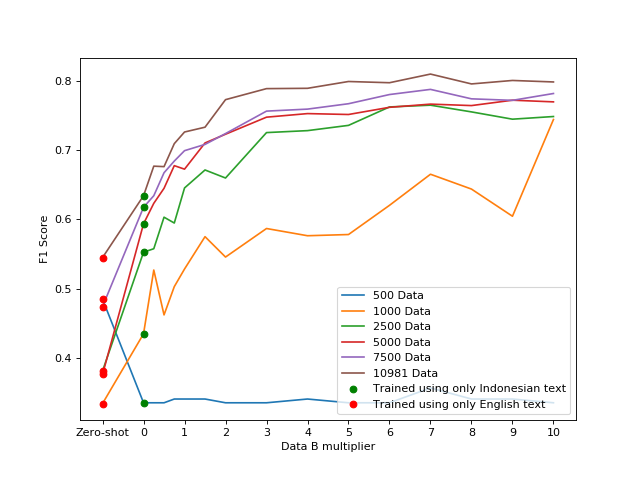
\includegraphics[width=0.75\textwidth]{resources/plot-head-prosa-xlmr.png}
                \caption{Plot dataset B dengan model XLM-R.}
                \label{fig:plot_head_prosa_xlmr}
            \end{figure}
            Dapat dilihat pada Gambar \ref{fig:plot_head_prosa_xlmr}, performa analisis sentimen dataset B sangat terbantu dengan penambahan data berbahasa Inggris. Di berbagai total data, penambahan bahasa Inggris menambah rata-rata F1-score sebesar 0.229. Penambahan performa terbesar diobservasi pada eksperimen dengan jumlah data yang sedikit. Performa model meningkat dari 0.734 pada skenario monolingual hingga mencapai 0.819 pada penambahan bahasa Inggris sebanya 7 kali lipat dari total bahasa Indonesianya.

            \item Analisis sentimen dengan data dataset A Advisor \\
            \begin{figure}[ht]
                \centering
                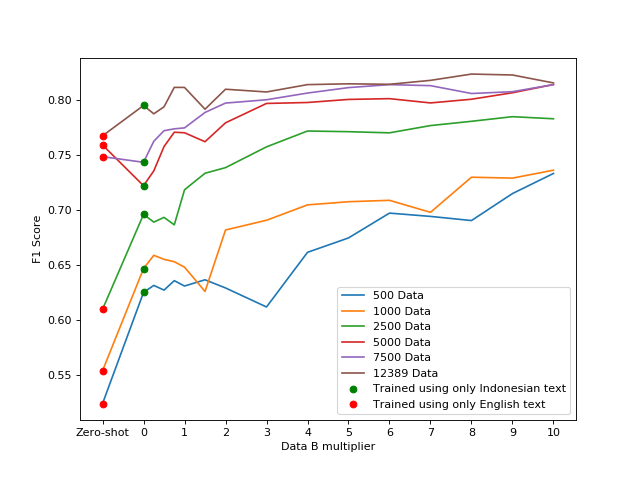
\includegraphics[width=0.75\textwidth]{resources/plot-head-trip-xlmr.png}
                \caption{Plot dataset A dengan model XLM-R.}
                \label{fig:plot_head_trip_xlmr}
            \end{figure}
            Dapat dilihat pada Gambar \ref{fig:plot_head_trip_xlmr}, performa analisis sentimen dataset A terbantu dengan penambahan data berbahasa Inggris. Di berbagai total data, penambahan bahasa Inggris menambah rata-rata F1-score sebesar 0.107. Penambahan performa terbesar juga diobservasi pada eksperimen dengan jumlah data yang sedikit. Performa model meningkat dari 0.794 pada skenario monolingual hingga mencapai 0.823 pada penambahan bahasa Inggris sebanya 8 kali lipat dari total bahasa Indonesianya.

            \item Klasifikasi ujaran kebencian \& kasar \\
            \begin{figure}[ht]
                \centering
                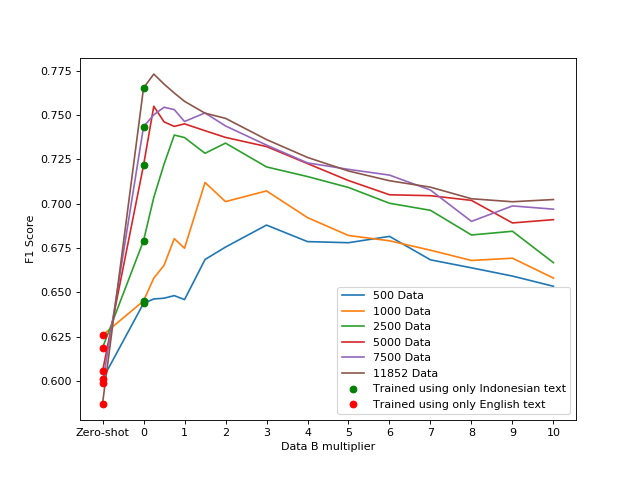
\includegraphics[width=0.75\textwidth]{resources/plot-head-toxic-xlmr.png}
                \caption{Plot klasifikasi ujaran kebencian dengan model XLM-R.}
                \label{fig:plot_head_toxic_xlmr}
            \end{figure}
            Dapat dilihat pada Gambar \ref{fig:plot_head_toxic_xlmr}, performa klasifikasi ujaran kebencian tidak terlalu terbantu dengan penambahan data berbahasa Inggris. Meski performa model sempat terbantu, penambahan lebih banyak data bahasa Inggris menurunkan performa model.

        \end{enumerate}
        
        Melalui rangkaian eksperimen dengan model XLM-R di atas, dapat dilihat korelasi antara perbedaan performa skenario \textit{zero-shot} dan \textit{monolingual} dengan performa skenario \textit{multilingual learning}. Eksperimen sentimen analisis dataset B memiliki rata-rata perbedaan skenario 1 dan 2 sebesar 0.0005. Dengan perbedaan yang sangat kecil, penambahan bahasa Inggris sangat bermanfaat. Eksperimen sentimen analisis dataset A memiliki rata-rata perbedaan skenario 1 dan 2 sebesar 0.044. Dengan perbedaan yang cukup besar, penambahan bahasa Inggris menjadi berkurang manfaatnya. Terakhir, eksperimen klasifikasi ujaran kebencian memiliki perbedaan skenario 1 dan 2 sebesar 0.093. Dengan perbedaan yang sangat besar, penambahan bahasa Inggris menjadi kurang bermanfaat dan bahkan menurunkan performa model.

        Berikut hasil eksperimen dengan model mBERT: 

        \begin{figure}[ht]
            \minipage{0.5\textwidth}
              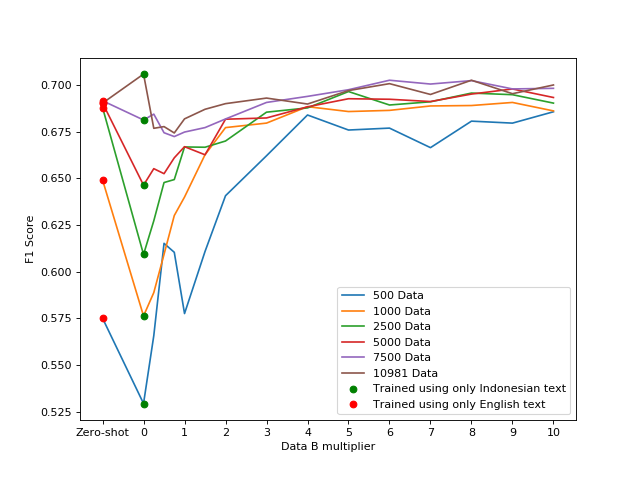
\includegraphics[width=\linewidth]{resources/plot-head-prosa-mbert.png}
              \caption{Plot dataset B model mBERT}\label{fig:plot_head_prosa_mbert}
            \endminipage\hfill
            \minipage{0.5\textwidth}
              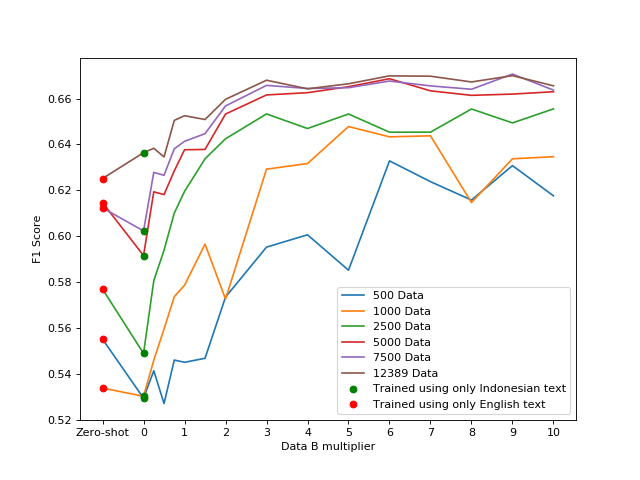
\includegraphics[width=\linewidth]{resources/plot-head-trip-mbert.png}
              \caption{Plot dataset A model mBERT.}\label{fig:plot_head_trip_mbert}
            \endminipage
        \end{figure}

        \begin{figure}[ht]
            \centering
            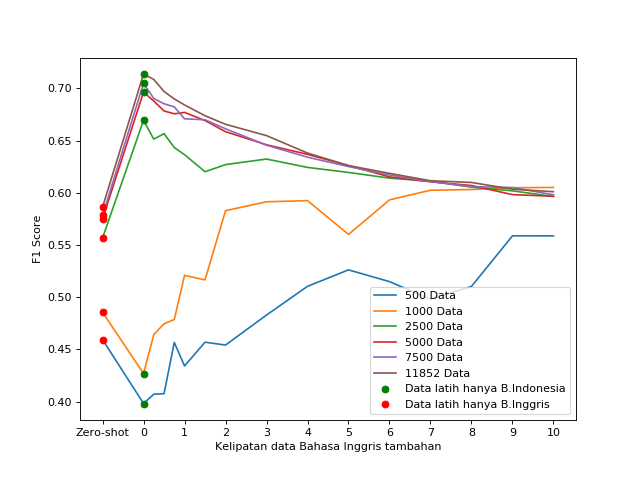
\includegraphics[width=0.5\textwidth]{resources/plot-head-toxic-mbert.png}
            \caption{Plot ujaran kebencian model mBERT.}\label{fig:plot_head_toxic_mbert}
        \end{figure}

        Melalui rangkaian eksperimen dengan model mBERT di atas, dapat dilihat hal yang sama dengan eksperimen model XLM-R. Secara umum performa mBERT lebih lemah dibanding XLM-R. Selain itu, dapat dilihat juga biasnya \textit{pretraining} mBERT ke bahasa Inggris. Di berbagai total data, performa \textit{zero-shot} lebih bagus dibanding pasangan \textit{monolingual}-nya. Hal ini dikarenakan dalam pelatihan mBERT memiliki jumlah data bahasa Inggris yang tidak proporsional dengan data lainnya. Berbeda dengan XLM-R yang melakukan \textit{sampling} pada tiap \textit{batch} pelatihannya untuk memastikan performa model proporsional antar bahasa.
            

    \subsection{Hasil fine-tune penuh}
        Eksperimen fine-tune penuh masih sedang dijalankan. Berikut hasil eksperimen yang sudah selesai dengan model XLM-R pada analisis sentimen dataset B dan klasifikasi ujaran kebencian :

        \begin{figure}[ht]
            \minipage{0.5\textwidth}
              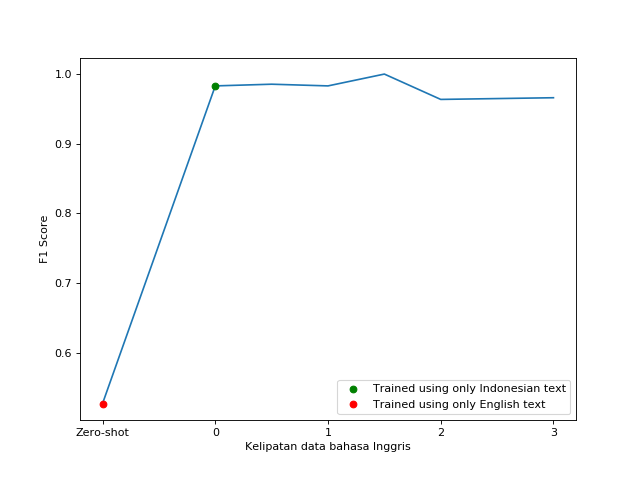
\includegraphics[width=\linewidth]{resources/plot-full-prosa-xlmr.png}
              \caption{Plot dataset A model XLM-R}\label{fig:plot_full_prosa_xlmr}
            \endminipage\hfill
            \minipage{0.5\textwidth}
              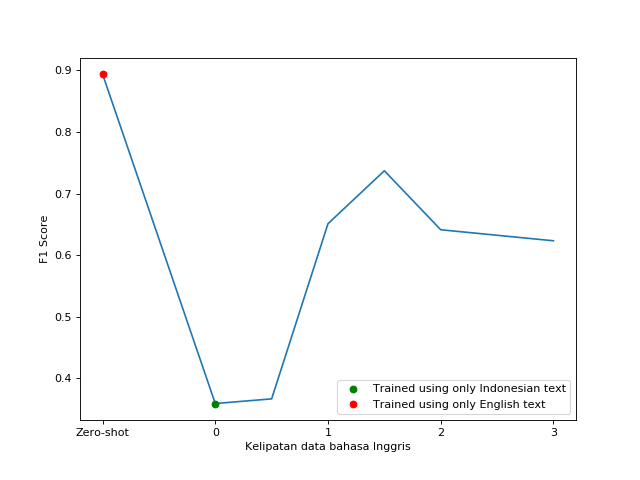
\includegraphics[width=\linewidth]{resources/plot-full-trip-advisor-xlmr.png}
              \caption{Plot dataset B model XLM-R}\label{fig:plot_full_prosa_xlmr}
            \endminipage
        \end{figure}

        \begin{figure}[ht]
            \minipage{0.5\textwidth}
                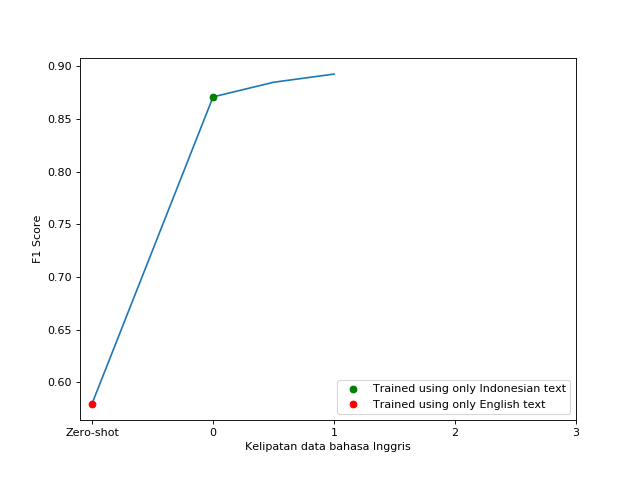
\includegraphics[width=\linewidth]{resources/plot-full-toxic-xlmr.png}
                \caption{Plot Ujaran kebencian model XLM-R.}\label{fig:plot_full_toxic_xlmr}
            \endminipage\hfill
            \minipage{0.5\textwidth}
                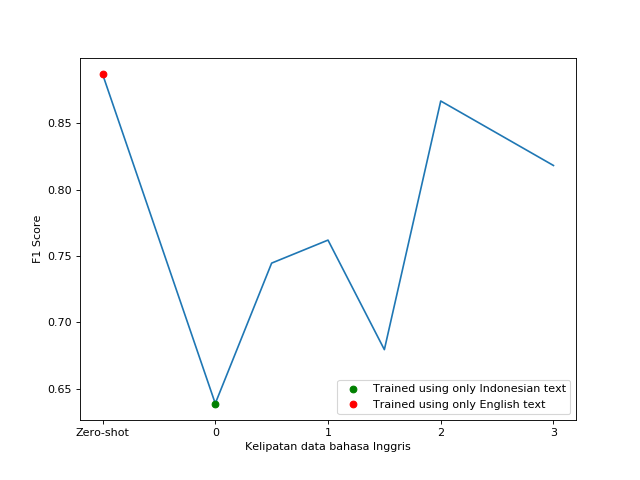
\includegraphics[width=\linewidth]{resources/plot-full-trip-advisor-xlmr-duplicate.png}
                \caption{Plot dataset A model XLM-R duplikat dihilangkan}\label{fig:plot_fuLL_trip_duplicate}
            \endminipage
        \end{figure}
        Melalui sedikit eksperimen dengan model XLM-R, dapat dilihat performa model XLM-R sangat bagus. Pada analisis sentimen dataset B model berhasil memprediksi seluruh data tes dengan sempurna di skenario 3 dengan kelipatan bahasa Inggris 1.5. Pada klasifikasi ujaran kebencian model berhasil mencapai F1-Score 0.892 di skenario 3 dengan kelipatan bahasa Inggris 1. 

        Meski begitu, pada analisis sentimen dataset A, model yang dilatih dengan bahasa Indonesia dan campuran memiliki performa yang jauh lebih jelek dibanding model yang dilatih dengan bahasa Inggris saja. Selain itu, hasil fine-tune penuh klasifikasi ujaran kebencian tidak dapat dibandingkan dengan penelitian sebelumnya secara langsung. Dua hal ini akan dibahas pada bab selanjutnya

\subsection{Analisis hasil}
    Sub bab ini akan membahas lebih detail hasil yang didapatkan pada bab sebelumnya

    \subsection{Hasil fine-tune penuh klasifikasi ujaran kebencian}
    Untuk dapat membandingkan secara langsung penggunaan \textit{multilingual language model}, pelatihan dengan konfigurasi yang sama dengan skenario 2 penelitian \parencite{Ibrohim_Budi_2019} dilakukan. Hasilnya dapat dilihat pada Tabel \ref{tab:toxic_xlm_r_comparable}.

    \begin{table}[]
        \centering
        \begin{tabular}{|r|l|l|l|}
        \hline
        \multicolumn{1}{|l|}{} & \textbf{Hate Speech} & \textbf{Abusive} & \textbf{Average}      \\ \hline
        \textbf{Accuracy}      & 85.573273\%          & 93.470008\%      & \textbf{89.5216405\%} \\ \hline
        \textbf{F1}            & 0.85331737           & 0.93094791       & \textbf{0.89213264}   \\ \hline
        \end{tabular}
        \caption{Hasil fine-tune penuh klasifikasi ujaran kebencian \textit{comparable}.}
        \label{tab:toxic_xlm_r_comparable}
    \end{table}

    \subsection{Hasil fine-tune penuh analisis sentimen data A}
    Setelah ditelusuri, ternyata dataset A memiliki 2573 teks duplikat. Sehingga, dari total 12389 data teks, hanya 9816 teks yang unik. Hal ini menyebabkan \textit{language model} overfit kepada data ini dan tidak mempelajari permasalahan secara sepenuhnya. Eksperimen fine-tune penuh analisis sentimen data A dijalankan kembali pada dataset yang dihilangkan teks duplikatnya. Hasilnya dapat dilihat pada Gambar \ref{fig:plot_fuLL_trip_duplicate}

    



    
        
